%SUPERFICIES FORESTALES

%----------------------------------------------------------
\section{Entorno de trabajo}

    El entorno de trabajo es el medio por el cual el usuario interactúa con el sistema para poder gestionar la información referente a la Escuela Libre de Derecho. En este capítulo se describe el comportamiento y los elementos que conforman el entorno de trabajo del SAEV2.0, como son: la disposición de los elementos principales y comunes de las pantallas, los colores, la iconografía, componentes, etc. \bigskip

    \begin{objetivos}
      \item Describir las áreas principales del entorno de trabajo.
      \item Describir la iconografía utilizada en las pantallas.
      \item Describir el mapa de navegación del sistema.
      \item Describir los componentes principales de las pantallas, tales como: controles de entrada, datos obligatorios, separadores, tablas de resultados, entre otros.
    \end{objetivos}
\\\\\\\\\\\\\\\\
%----------------------------------------------------------

\subsection{Diseño}

  El diseño de las pantallas del sistema sigue un enfoque minimalista que permite a los usuarios trabajar sin gran dificultad y sin distracción. 
  Las pantallas son consistentes, ya que tienen un diseño homogéneo y cuentan con componentes comunes; la consistencia facilita al usuario la interacción
  con el sistema a medida que hace uso del mismo. En la figura~\ref{fig:entornoDeTrabajo} se muestran los elementos principales que conforman las pantallas del sistema, 
  dichos elementos se describen a continuación:

  \begin{figure}[ht!]
      \begin{center}
	  \fbox{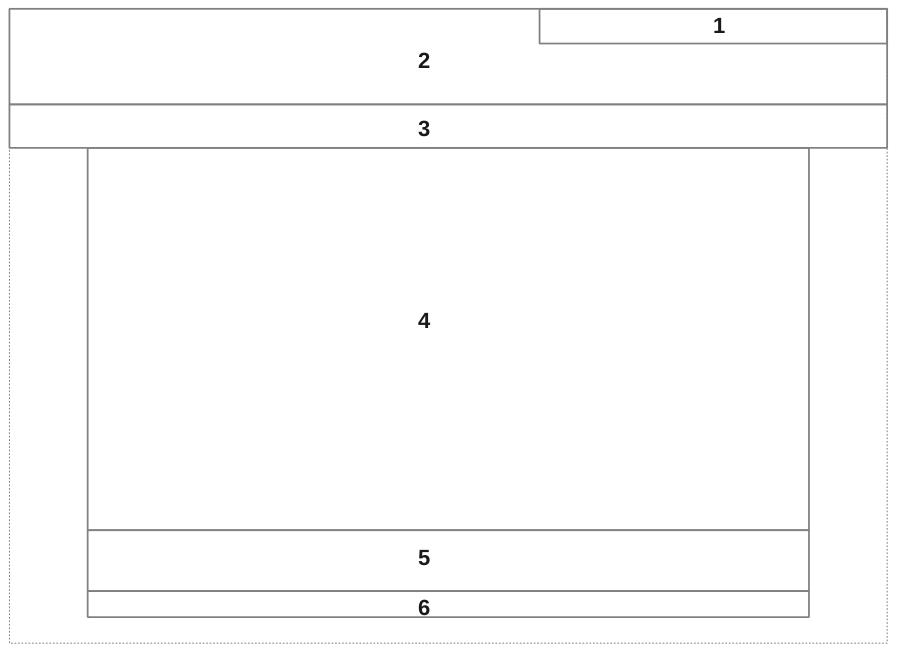
\includegraphics[width=.8\textwidth]{images/pantallas/general/entornoTrabajo.png}}
	  \caption{Entorno de trabajo del sistema.}
	  \label{fig:entornoDeTrabajo}
      \end{center}
  \end{figure}

    \begin{enumerate}
        \item {\bf Encabezado:} el encabezado tiene la finalidad de mostrar la imagen institucional de la dependencia a la cual pertenece, es decir, la imagen institucional del Gobierno del Estado de México.
        \begin{itemize}
            \item Ancho: $100\%$ del ancho de la ventana del navegador.
            \item Alto: $90px$.
        \end{itemize}

        \item {\bf Menú horizontal:} muestra las opciones generales de navegación para los distintos tipos de usuarios.
        \begin{itemize}
            \item Ancho: $100\%$ del ancho de la pantalla del navegador.
            \item Alto: $40px$.
        \end{itemize}
        
        \item {\bf Menu vertical:} es el área destinada al menú vertical que contendrá los vínculos necesarios para ingresar a las opciones que proporcione el sistema a cada uno de los distintos perfiles de usuarios.
        
        El menú vertical no se encontrará visible para los perfiles de usuario que no requieran del mismo y este espacio será utilizado por el área de trabajo (ver siguiente punto).
        
        \begin{itemize}
            \item Ancho: $20\%$ del ancho de la pantalla del navegador.
            \item Alto: autoajustable al contenido.
        \end{itemize}
        
        \item {\bf Área de trabajo:} en esta sección los usuarios visualizarán los elementos que el sistema proporciona para la realización de las tareas contempladas en el mismo. Aquí se desplegarán formularios para captura, tablas, imágenes, gráficas y demás elementos contenidos en el sistema.\\
        
        El contenido en esta sección se visualizará centrada con base en el ancho y alineado a la parte superior de la misma. Todas las pantallas deberán contar con un título alineado al centro del área de trabajo. 
        \begin{itemize}
            \item Ancho: ancho mínimo $500px$, $65\%$ del ancho de la ventana del navegador web cuando el menu vertical esta visible o el $80\%$ del ancho de la ventana del navegador web en ausencia del menu vertical.
            \item Alto: autoajustable al contenido con un mínimo de $400px$.
        \end{itemize}
        
        \item {\bf Pie:} esta sección contendrá la información de contacto de la unidad correspondiente de la Secretaría del Medio Ambiente del Gobierno del Estado de México.
        \begin{itemize}
            \item Ancho: $80\%$ del ancho de la ventana del navegador.
            \item Alto: $84px$
        \end{itemize}
        
        \item {\bf Información legal:} muestra una leyenda con información legal referente a la propiedad y uso del sistema.
        \begin{itemize}
            \item Ancho: $100\%$ del ancho de la ventana del navegador.
            \item Alto: 24px.
        \end{itemize}
        
        \item {\bf Información de sesión:} esta sección será visible sólo cuando un usuario ingrese al sistema. En ella se mostrarán las opciones para cambiar la contraseña de acceso al mismo, el nombre de usuario y el cierre de sesión.
        \begin{itemize}
            \item Ancho: ajustable al contenido.
            \item Alto: $30px$;
        \end{itemize}
    \end{enumerate}

  
%\subsection{Pantalla de bienvenida}
%\label{ch:Interaccion:PantallaBienvenida}


%----------------------------------------------------------

%\subsection{Componentes utilizados}

 % \subsubsection{Pantalla emergente}
  
  
%----------------------------------------------------------
%\subsection{Datos de sesión}
%\label{ch:Interaccion:DatosSesion}


%\subsection{Iconografía}

%  En las pantallas se utilizan diversos íconos para denotar las operaciones que el actor puede realizar sobre el sistema. Los íconos se diseñaron con base en los perfiles de actor y en la operación que podrán realizar 
%  después del evento {\it clic} sobre ellos.  A continuación se describe la la funcionalidad de cada uno de ellos:\\\\

%  \begin{UClist}
    %\UCli \botKo: Permite eliminar un registro del sistema, por ejemplo: un integrante de línea de acción, una actividad en el plan de acción, etc. Al utilizar este ícono no se podrá recuperar la información eliminada. 
%    \UCli \botOk: Se utiliza para aprobar la solicitud de inscripción de una escuela al programa.
%     \UCli \botReg Se utiliza para solicitar el registro de información en el sistema, por ejemplo: un nuevo integrante de línea de acción, información correspondiente al diagnoóstico, etc. 
  %    \end{UClist}


%----------------------------------------------------------
  
\subsection{Organización}
Las funcionalidades del sistema se encuentra organizadas por menús. Cada actor accede a un menú diferente dependiendo de su perfil, ya que este describe el ciclo de trabajo y las funciones que el actor puede realizar.


\hypertarget{menu:SP-MenuEA}{}	
\subsection{Menú Principal: Secretaría de Posgrado}
En la figura \ref{MN1} se muestran el menú mediante el cual la Secretaría Posgrado puede acceder a sus funcionalidades.
\IUfig[.2]{menus/SP.png}{MN1}{Menú de la Secretaría de Posgrado}

\hypertarget{submenu:SP-MenuDiplomado}{}	
\subsection{Submenú Diplomado: Secretaría de Posgrado}
En la figura \ref{MN2} se muestran el submenú mediante el cual la Secretaría de Posgrado puede acceder a las funcionalidades correspondientes a un diplomado.
\IUfig[.2]{menus/SP-Diplomado.png}{MN2}{Submenú Diplomado de la Secretaría de Posgrado}

\hypertarget{submenu:SP-MenuEspecialidad}{}	
\subsection{Submenú Especialidad: Secretaría de Posgrado}
En la figura \ref{MN3} se muestran el submenú mediante el cual la Secretaría de Posgrado puede acceder a las funcionalidades correspondientes a una especialidad.
\IUfig[.2]{menus/SP-Especialidad.png}{MN3}{Submenú Especialidad de la Secretaría de Posgrado}

\hypertarget{submenu:SP-MenuMaestria}{}	
\subsection{Submenú Maestría: Secretaría de Posgrado}
En la figura \ref{MN4} se muestran el submenú mediante el cual la Secretaría de Posgrado puede acceder a las funcionalidades correspondientes a una maestría.
\IUfig[.2]{menus/SP-Maestria.png}{MN4}{Submenú Maestría de la Secretaría de Posgrado}

\hypertarget{menu:CCE-MenuEA}{}	
\subsection{Menú Principal: Coordinación de Control Escolar/Directora Académica}
En la figura \ref{MN5} se muestran el menú mediante el cual la Coordinación de Control Escolar o la Directora Académica pueden acceder a las funcionalidades del sistema.
\IUfig[.2]{menus/CCE.png}{MN5}{Menú de la Coordinación de Control Escolar/Directora Académica}

\hypertarget{submenu:CCE-MenuDiplomado}{}	
\subsection{Submenú Diplomado: Coordinación de Control Escolar/Directora Académica}
En la figura \ref{MN6} se muestra el submenú mediante el cual la Coordinación de Control Escolar o la Directora Académica pueden acceder a las funcionalidades correspondientes a los programas académicos de diplomado.
\IUfig[.2]{menus/CCE-Diplomado.png}{MN6}{Submenú Diplomado de la Coordinación de Control Escolar/Directora Académica}

\hypertarget{submenu:CCE-MenuEspecialidad}{}	
\subsection{Submenú Especialidad: Coordinación de Control Escolar/Directora Académica}
En la figura \ref{MN7} se muestran el submenú mediante el cual la Coordinación de Control Escolar o la Directora Académica pueden acceder a las funcionalidades correspondientes a los programas académicos de especialidad.
\IUfig[.2]{menus/CCE-Especialidad.png}{MN7}{Submenú Especialidad de la Coordinación de Control Escolar/Directora Académica}

\hypertarget{submenu:CCE-MenuMaestria}{}	
\subsection{Submenú Maestría: Coordinación de Control Escolar/Directora Académica}
En la figura \ref{MN8} se muestran el submenú mediante el cual la Coordinación de Control Escolar o la Directora Académica pueden acceder a las funcionalidades correspondientes a un programa académico de maestría.
\IUfig[.2]{menus/CCE-Maestria.png}{MN8}{Submenú Maestría de la Coordinación de Control Escolar/Directora Académica}

\hypertarget{submenu:SP-Inscripcion}{}	
\subsection{Submenú Inscripción: Secretaría de Posgrado}
En la figura \ref{MN9} se muestran el submenú mediante el cual la Secretaría de Posgrado puede acceder a las funcionalidades correspondientes a la inscripción de aspirantes a un programa académico.
\IUfig[.2]{menus/SP-Inscripcion.png}{MN9}{Submenú de Inscripción}